\chapter{Resultados Preliminares}

\section{Caracterização das membranas}

O processo de caracterização das membranas gerou como resultado as informações sobre diâmetro de poro médio, diâmetro máximo, ângulo de contato e LEP. Dentre as membranas testadas, as membranas M4 e M6 apresentaram diâmetros de poro médio com aproximadamente uma ordem de grandeza superior as demais. A incerteza associada aos diâmetros de poro foi calculada considerando que os dados possuem uma distribuição normal. Uma análise estatistica mais aprofundada será realizada posteriormente para uma análise de incerteza mais acertiva. A figura \ref{fig:diamporo} apresenta os diâmetros de poro médio das membranas estudadas. As figuras \ref{fig:distporo1} e \ref{fig:distporo2} apresentam as distribuições de poro obtidas.

\begin{figure}[H]
    \centering
    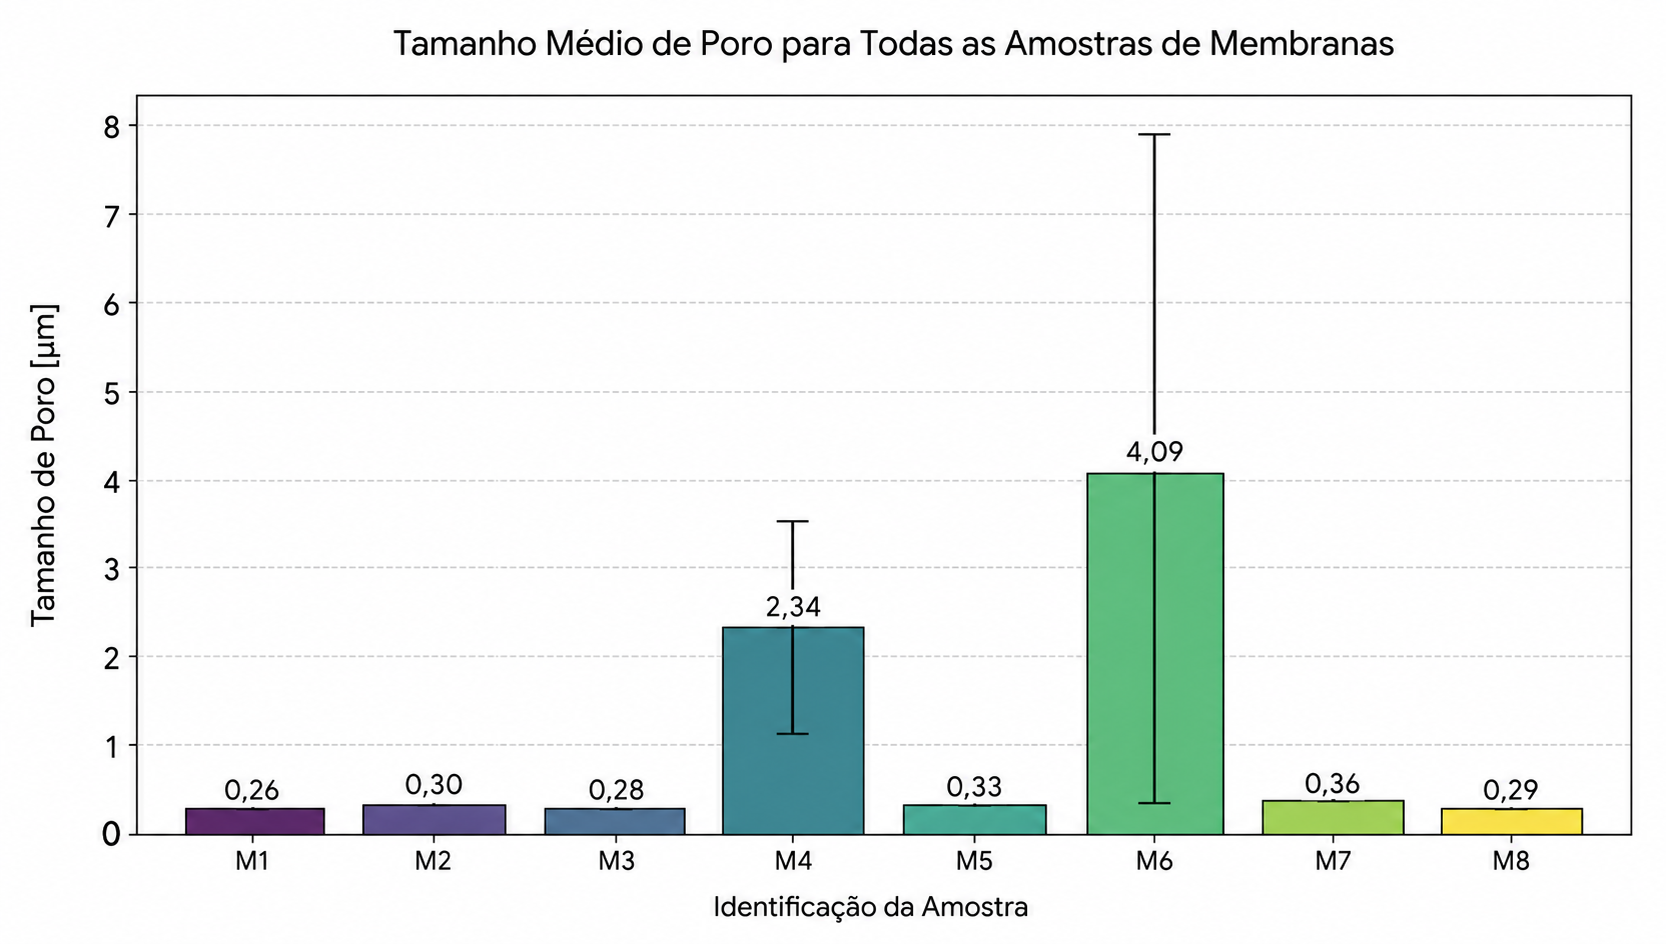
\includegraphics[width=\textwidth, height=8cm, keepaspectratio]{diametrodeporo.png}
    \caption{Diâmetro de poro médio das membranas analisadas, obtidos através de porosimetria de fluxo capilar.}
    \label{fig:diamporo}
\end{figure}

\begin{figure}[H]
    \centering
    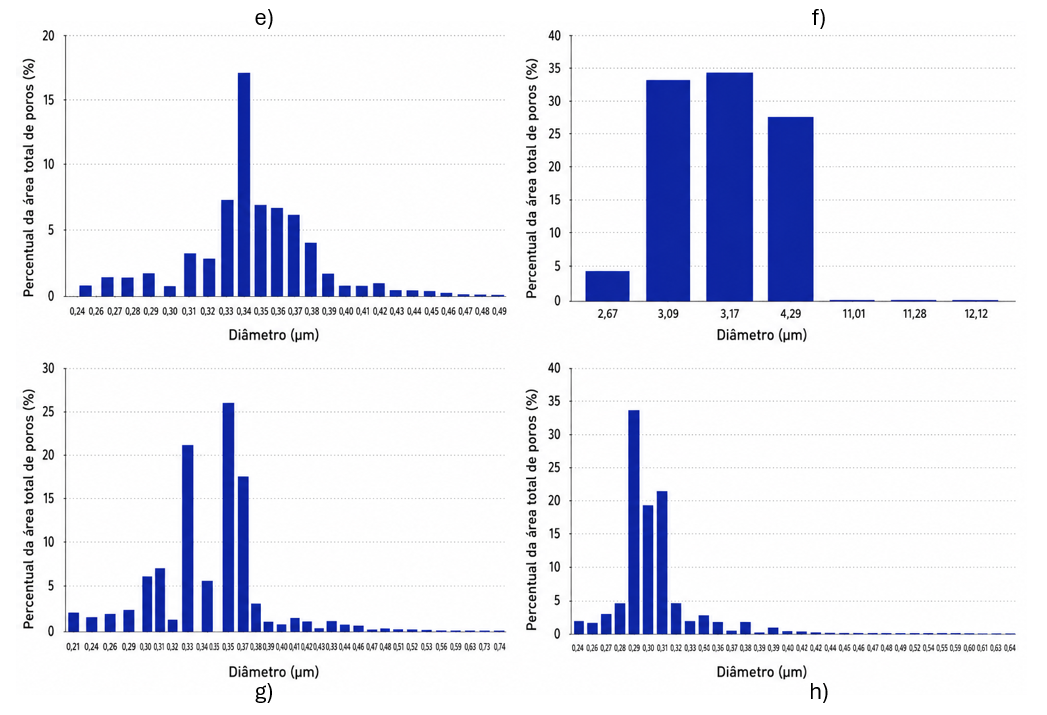
\includegraphics[width=\textwidth, height=12cm, keepaspectratio]{distporom5m8.png}
    \caption{Distribuições do diâmetro de poros obtidas para as membranas M1 a), M2 b), M3 c) e M4 d). }
    \label{fig:distporo1}
\end{figure}

\begin{figure}[H]
    \centering
    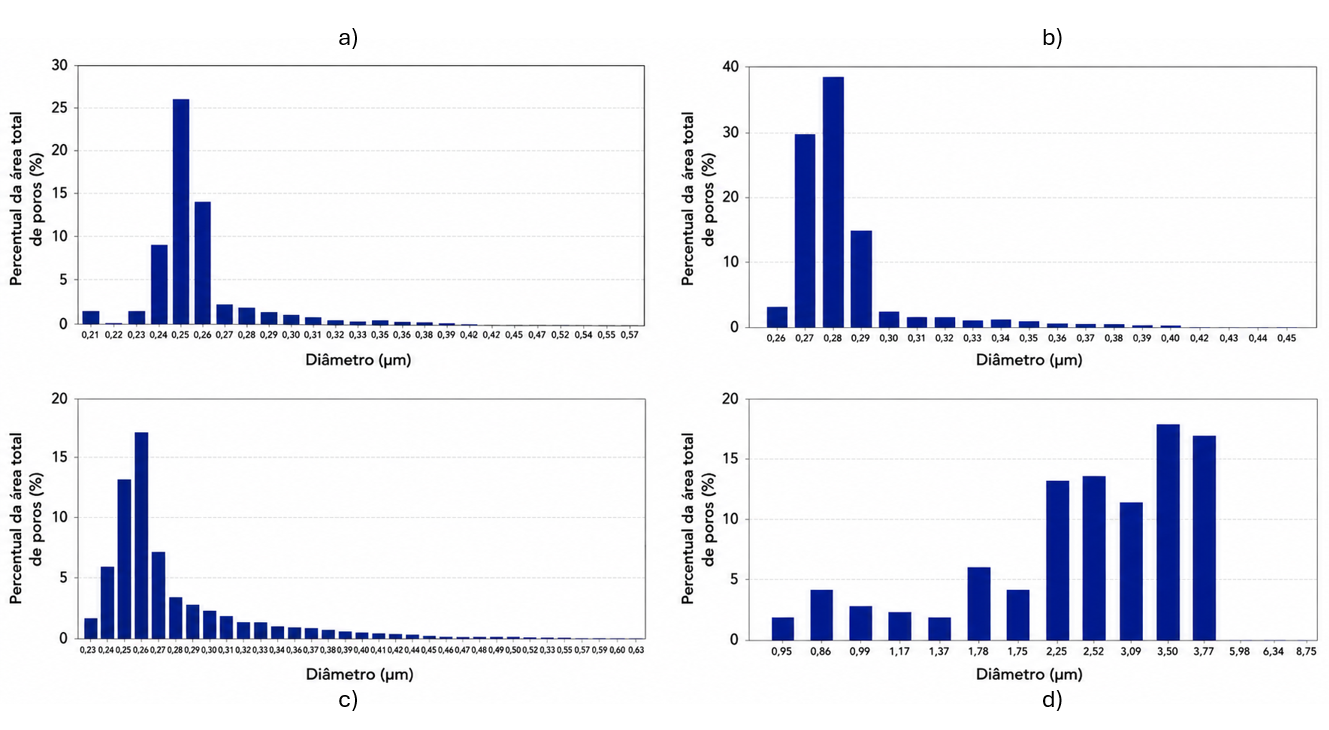
\includegraphics[width=\textwidth, height=12cm, keepaspectratio]{distporom1m4.png}
    \caption{Distribuições do diâmetro de poros obtidas para as membranas M5 a), M6 b), M7 c) e M8 d). }
    \label{fig:distporo2}
\end{figure}

As medições de ângulo de contato indicaram que as membranas encontram-se dentro da faixa hidrofóbica requerida para o processo de destilação por membranas. A figura \ref{fig:angulodecontato} apresentam as medições de ângulo de contato realizadas.

\begin{figure}[H]
    \centering
    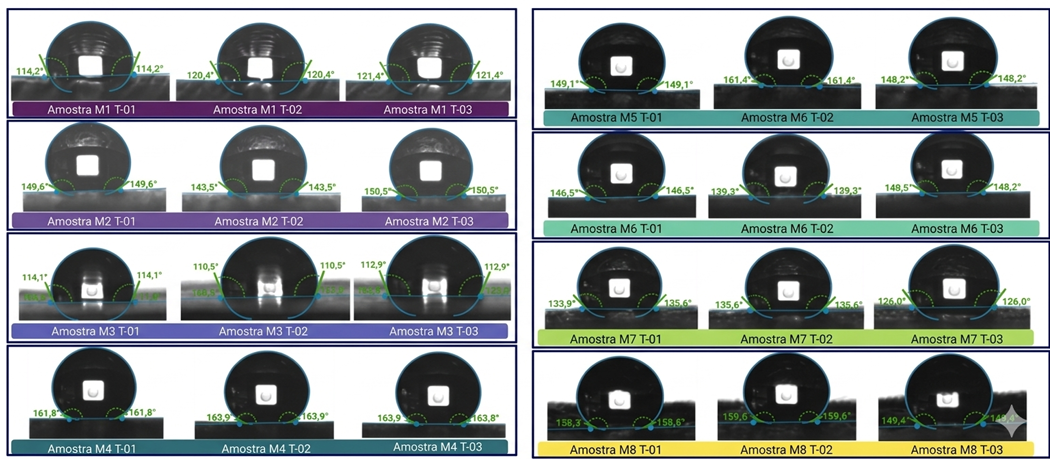
\includegraphics[width=\textwidth, height=12cm, keepaspectratio]{angulodecontato.png}
    \caption{Medições de ângulo de contato das membranas estudadas.}
    \label{fig:angulodecontato}
\end{figure}

Com base nos resultados obtidos nas análises de porosimetria e ângulo de contato, calculou-se o LEP utilizando a equação \ref{eq:LEP}.

\begin{figure}[H]
    \centering
    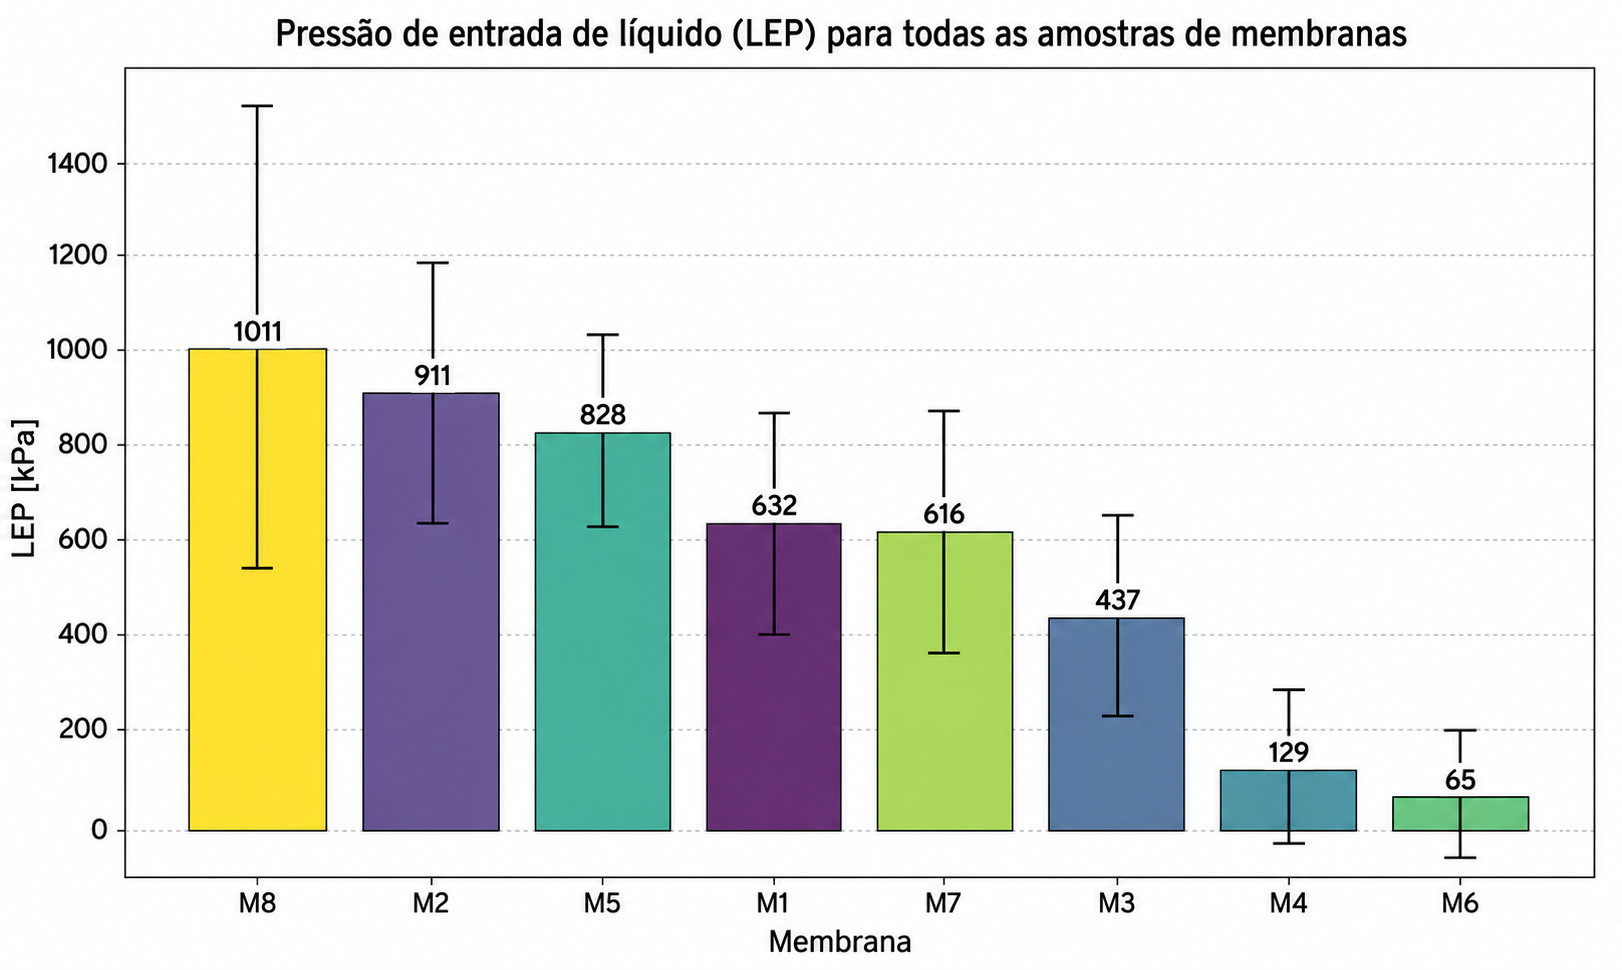
\includegraphics[width=\textwidth, height=12cm, keepaspectratio]{LEP.png}
    \caption{LEP calculado para as membranas estudadas.}
    \label{fig:angulodecontato}
\end{figure}